% Chapter 4

\chapter{Tools and Utilities} % Main chapter title

\label{Chapter4} % For referencing the chapter elsewhere, use \ref{Chapter4} 

\lhead{Chapter 4. \emph{Tools and Utilities}} % This is for the header on each page - perhaps a shortened title

%----------------------------------------------------------------------------------------

\section{JSON(JavaScript Object Notation)}
\subsection{Language Overview}
JSON \cite{JSON-standard} (JavaScript Object Notation) is a lightweight data-interchange format.It is easy for humans to read and write. It is easy for machines to parse and generate. It is based on a subset of the JavaScript Programming Language.JSON is a text format that is completely language independent but uses conventions that are familiar to programmers of the C-family of languages, including C, C++, C\#, Java, JavaScript, Perl, Python, and many others. These properties make JSON an ideal data-interchange language.

JSON has only two structures:
\begin{enumerate}
\item A collection of name/value pairs. In various languages, this is realized as an object, record, struct, dictionary, hash table, keyed list, or associative array.
\item An ordered list of values. In most languages, this is realized as an array, vector, list, or sequence.
\end{enumerate}
These are universal data structures. Virtually all modern programming languages support them in one form or another. It makes sense that a data format that is interchangeable with programming languages also be based on these structures.

In JSON, they take on these forms:
\begin{enumerate}
\item An object is an unordered set of name/value pairs. An object begins with \{ (left brace) and ends with \} (right brace). Each name is followed by : (colon) and the name/value pairs are separated by , (comma).
\item An array is an ordered collection of values. An array begins with [ (left bracket) and ends with ] (right bracket). Values are separated by , (comma).
\item A value can be a string in double quotes, or a number, or true or false or null, or an object or an array. These structures can be nested.
\item A string is a sequence of zero or more Unicode characters, wrapped in double quotes, using backslash escapes. A character is represented as a single character string. A string is very much like a C or Java string.
\item A number is very much like a C or Java number, except that the octal and hexadecimal formats are not used.
\item Whitespace can be inserted between any pair of tokens. Excepting a few encoding details, that completely describes the language.
\end{enumerate}

\subsection{json-simple(Parser API)}
JSON.simple\cite{JSON-simple} is a simple Java toolkit for JSON by google.
It has following features:
\begin{itemize}
\item Full compliance with JSON specification (RFC4627) and reliable (see compliance testing).
\item Provides multiple functionalities such as encode, decode/parse and escape JSON text while keeping the library lightweight.
\item Flexible, simple and easy to use by reusing Map and List interfaces.
\item Supports streaming output of JSON text.
\item Stoppable SAX-like interface for streaming input of JSON text (learn more).
\item Heap based parser.
\item High performance (see performance testing).
\item No dependency on external libraries.
\item Both of the source code and the binary are JDK1.2 compatible.
\end{itemize}

\section{Formats}
\subsection{Input File Format}
There will be two files coming in to the project, the sequence file stating the run sequences of the system. Each run system is described by the function calls called in order for that particular run. They are denoted by number here which is mapped in another file with the other details like the method name and class name. It is possible that the same method be called multiple amounts of time in a single run and thus a counter number is associated to uniquely identify the method at that position.

\begin{enumerate}
\item Method Trace:

[\{"counter": 0, "class-name": "com.ser.instrument.artifacts.InstrumentClass1", "method-name": "int methodWithPrimitiveInt(int)", "level": 28\},\\
 \{"counter": 1, "class-name": "com.ser.instrument.artifacts.InstrumentClass1", "method-name": "int methodWithPrimitiveInt(int)", "level": 29\}\\
]

\item Sequence Map File:

[\{"sequence-no":1, "counters" : [ 1,2, 3, 4, 5, 6, 7, 8, 9, 10]\},\\
 \{"sequence-no": 2, "counters" : [ 5, 7, 8, 10, 13, 15]\}\\
]

\end{enumerate}

\subsection{Output File Format}
There will be one output file generated which will have the frequent sequences for each run provided in the input file.
This basically is an array for each frequent sequence(here called method-sequence). With each frequent sequence we attach the counters at each run sequence.

Output:

[ \{"method-sequence" : [ 1, 3, 4 ],\\
\tab   "occurences" :\\
\tab\tab             { [\{ "sequence-no" : 1,\\
\tab\tab               "counters" : [ 100, 102, 103] \},\\
\tab\tab              \{ "sequence-no":  2,\\
\tab\tab                "counters" : [ 100, 102, 105] \},\\
\tab\tab                \{ "sequence-no" : 3,\\
\tab\tab                  "counters" : [ 500, 501, 510] \}\\
\tab\tab                  ]}\},\\
\\
  \{"method-sequence" : [ 8 ,9, 10 ],\\
\tab   "occurences" :\\
\tab\tab             { [\{ "sequence-no" : 8,\\
\tab\tab                "counters" : [ 100, 102, 103] \},\\
\tab\tab                \{ "sequence-no":  9,\\
\tab\tab                "counters" : [ 100, 102, 105] \},\\
\tab\tab                \{ "sequence-no" : 10,\\
\tab\tab                  "counters" : [ 500, 501, 510] \}\\
\tab\tab                  ]}\}\\
]

%----------------------------------------------------------------------------------------
\section{Maven}
\subsection{Overview}
Maven\cite{Maven} is a build tool made available by Apache. There are various uses of this tool as described below:

\begin{itemize}
\item Making the build process easy.
\item Providing a uniform build system.
\item Providing quality project information.
\item Providing guidelines for best practices development.
\item Allowing transparent migration to new features.
\end{itemize}

\subsection{Project Hierarchy}
Maven provides a well organized heirarchy for the project separating test and source folders in test and main folders.
The snapshot of the project heirarchy is shown in Fig.\ref{heirarchy}.

\begin{figure}[h]
\centering
 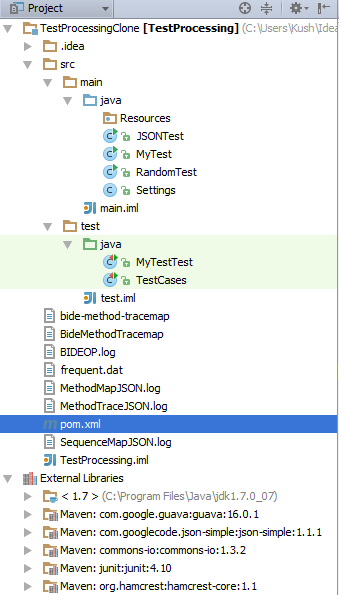
\includegraphics{maven_heirarchy}
\caption{Project Heirarchy.}
\label{heirarchy}
\end{figure}

\subsection{Project Object Model}
A Project Object Model or POM\cite{pom} is the fundamental unit of work in Maven. It is an XML file that contains information about the project and configuration details used by Maven to build the project. It contains default values for most projects. Examples for this is the build directory, which is target; the source directory, which is src/main/java; the test source directory, which is src/main/test; and so on.\\

The main use of the file is to include jar files of external resources like json parser, junit, etc. The build tool fetches the jars from the internet and is thus useful while collaborating as only pom.xml can be shared instead of the physical jar themselves.\\


Following Fig.\ref{pom} is the pom.xml for the project:
\begin{figure}[h]
\centering
 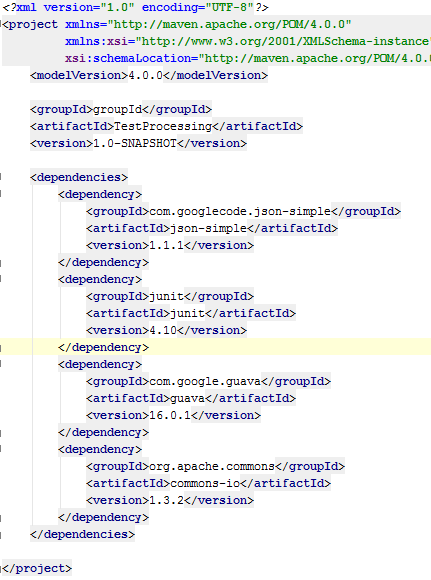
\includegraphics{maven_pom}
\caption{pom.xml.}
\label{pom}
\end{figure}

\section{BIDE (BI-Directional Extension based frequent closed sequence mining)}
\subsection{Overview}
The goal of using this tool is to mine frequent patterns of method invocations invoked in execution traces that were collected by the profiler from the AUT with acceptance and get models of interactions among different components.

Frequent patterns are sequences occuring in the dataset more than a predefined and user defined threshold value\cite{Han:2007:FPM:1275092.1275097}.

For example, a person visits a mall every week and buys some items. He will have a list of items that he bought, suppose each as a row in the dataset. If for assumption, milk and bread appear more than the threshold value, in the rows, they are called as Frequent Sequential Pattern.

 \{1 2 4 10\} is a frequent sequence in a following run sequence \{1 2 4 10 12 3 5 7 4 2 7 4 8 10\} 
 This sequence is closed and maximal because they are the biggest sequences that are not present in larger and equally or higher frequent sequences.
 
 Thus, we need a miner developed by academicians from University of Illinois at Urbana- Champagne \cite{Wang:2004:BEM:977401.978142}
 It is a very easy to use executable which can be used by accessing the operating system process for running it.
 
 Let us go through the details of using BIDE:
 
\subsubsection{Input parameters}
\tab1st argument: The specification file of the dataset\\
\tab2nd argument: Relative support in decimal\\
Usage example: bide $bide_input$.spec 0.0002\\
Where bide is the executable file name, $bide_input$.spec is the specification file of the sequence dataset being mined, 0.0002 is the relative support.
As to the dataset file format, see section 4.4.1.4.

\subsubsection{Output}
The discovered frequent sequences are printed into a file called “frequent.dat”.\\
Each line in the result file, “frequent.dat”, contains a frequent sequence in the form:\\
event1 event2 … eventn : absolute support\\
Here is an example:\\
6 24 748 : 66\\


\subsubsection{Specification file format}
The first line is the dataset file name.\\
The second line is the number of unique items.\\ 
The third line is the number of sequences.\\ 
The fourth line is the maximal length of a sequence.\\
The fifth line is the average length of a sequence.

\subsubsection{Dataset file format}
Usually a sequence database consists of a series of sequences (strictly speaking, here a sequence is a string in the current implementation). Each line represents a sequence and ends with -1, and the entire dataset ends with -2.\\
Here is a sample sequence:\\
In our case each number is an item in run sequence more precisely a function invocation.\\
And each line represents a different run sequence.\\
For eg.\\
1 4 35 90 -1\\
1 2 3 54 77 -1\\
-2

\subsection{Other Tools}
\begin{enumerate}
\item Java Standard Edition Development Kit 7 for coding. 
\item IntelliJ (Intgrated Development Environment).
\item HP-ENVY 4 Laptop for all the experiments.
\item GitHub online repository for collaboration.
\item Tortoise SVN for version control.
\end{enumerate}


